% \documentclass[12pt,openright,oneside,a4paper,brazil]{abntex2}
% \usepackage[utf8]{inputenc}
% \counterwithout{section}{section}
% \counterwithout{figure}{chapter}
% \counterwithout{table}{chapter}
% \setlength{\parindent}{1.3cm}
% \usepackage{indentfirst}
% \setlength{\parskip}{0.2cm}
% \usepackage[bottom=2cm,top=3cm,left=3cm,right=2cm]{geometry}
% \usepackage{graphicx}
% \graphicspath{{figuras/}}
% \usepackage{placeins}
% 
% %opening
% \title{}
% \author{}
% 
% \begin{document}
% 
% 
% \textual
\begin{center}
 {\large Plano de gerenciamento de riscos}\\[0.2cm]
 {Planta de abastecimento de água potável a partir da umidade do ar}\\
 \end{center}
 
 \section{Histórico de Alterações}
\begin{table}[h]
\centering
\begin{tabular}{|c|c|p{6cm}|p{5cm}|}

Data & Versão & Descrição & Responsável\\
\hline                               
17/04/2015 & 0.0 & Criação do Plano de Gerenciamento das comunicações & Cesar Antonio Marques Junior, Jonnatas Lennon Lima Costa, Victor Borges.
\\
\hline
24/04/2015 & 1.0 & Alteração nos itens VII, VII e X & Cesar Antonio M. Júnior.\\
\hline
\end{tabular}
\end{table}

\section{Objetivo}
O objetivo desse plano é estabelecer um processo de gerenciamento de riscos do projeto.

\section{Descrição dos processos de gerenciamento de riscos}
Dentre os processos de gerenciamento de riscos deve-se frisar pela identificação e  analise qualitativa dos riscos, para assim obter ferramentas de respostas eficazes aos ricos evidentes, assim sendo os artefatos gerados neste projeto serão.
\begin{itemize}
\item Plano de gerenciamento de risco.
\item Identificação de risco.
\item Analise quantitativa de risco.
\item Analise qualitativa de tisco.
\item Planejamento de resposta aos riscos.
\end{itemize}

\section{EAR – Estrutura Analítica de Riscos para identificação dos riscos}
\begin{figure}[h]
\begin{center}

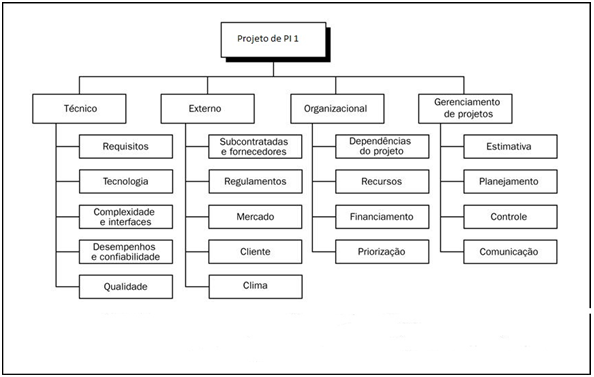
\includegraphics[scale=0.65]{editaveis/figuras/ear}
\label{ERR}

\end{center}
\end{figure}
\FloatBarrier

\section{Qualificação dos riscos}
Os riscos identificados serão qualificados na sua probabilidade de ocorrência e impacto nos resultados, conforme tabela a seguir:

Probabilidade:
\begin{table}[h]
\centering
\begin{tabular}{|c|c|c|}

  & Nível & Descrição\\
\hline                               
1 & baixa & Impedimento devido a licenças ambientais. \\
\hline
2 & alta & Alto custo dos componentes integrantes no aparelho.\\
\hline
3 & alta & Pouco tempo para o desenvolvimento de um projeto altamente complexo.\\
\hline
4 & media & Pouca vasão de agua gerada, pelo aparelho. \\
\hline
\end{tabular}
\end{table}

Impacto:
\begin{table}[h]
\centering
\begin{tabular}{|c|c|p{13.3cm}|}

  & Nível & Descrição\\
\hline                               
1 & alta & Caso ocorra havera a paralização da execução do projeto. \\
\hline
2 & alta & Caso ocorra podera inviabilizar o projeto devido o alto custo do aparelho a ser desenvolvido.\\
\hline
3 & alta & Não ocorrerar grande impactos no projeto.\\
\hline
4 & media & Ocorrerar inviabilidade finaceira sobre a implementação. \\
\hline
\end{tabular}
\end{table}

Prioridade: Probabilidade X Impacto
\begin{figure}[h]
\begin{center}

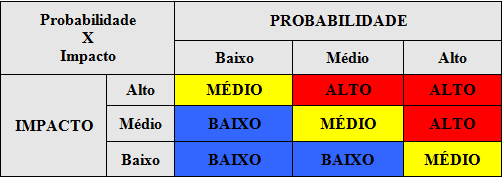
\includegraphics[scale=0.65]{editaveis/figuras/prioridade}
\label{Prioridade}
\end{center}
\end{figure}
\FloatBarrier

\section{Quantificação dos riscos}
Análise quantitativa dos riscos tem como objetivo mensurar a probabilidade de ocorrência dos riscos, suas conseqüências e estimar as implicações no projeto.

A análise quantitativa de riscos deve ser repetida após o planejamento de respostas a riscos, e também como parte do monitoramento e controle de riscos, para determinar se o risco total do projeto diminuiu de forma satisfatória. As tendências podem indicar uma necessidade de aumento ou diminuição das ações de gerenciamento de riscos.

Serão usadas técnicas como a análise de árvore de decisão e a simulação de Monte Carlo para:
\begin{itemize}
\item Quantificar os possíveis resultados do projeto e suas probabilidades.
\item Avaliar a probabilidade de atingir objetivos específicos do projeto.
\item Identificar os riscos que exigem mais atenção quantificando sua contribuição relativa para o risco total do projeto.

\end{itemize}

\section{Sistema de Controle de mudanças de riscos}
As mudanças surgirão basicamente da comparação dos resultados obtidos com os resultados esperados. Durante as reuniões os pontos analisados são levantados para discussão entre os integrantes do grupo, dessa forma o resposável por tal atividade e os envolvidos poderão buscar a melhor alternativa de contenção para os riscos avaliados. 

\section{Reserva de contingência}
\begin{table}[h]
\centering
\begin{tabular}{|c|c|}
Cargo & Reservas de contingência\\
\hline
Gerente de projeto & Até R\$ 2.000\\
\hline
Compras com equipamentos & Até R\$ 3.000\\
\hline
Pesquisa e desenvolvimento & Até R\$ 500\\
\hline
\end{tabular}
\end{table}

Esta autonomia baseia-se na nas diretrizes do plano de gerenciamento dos riscos, de modo à oferecer uma resposta rápida, as ações que ocasionariam algum risco, com base em ocorrência das ações. 
\section{Frequência de avaliação dos riscos do projeto}
Seguindo o cronograma de atividades do projeto, a avaliação dos riscos será feita conforme a entrega das atividades de cada área do projeto, estando sujeita à aprovação dos envolviodos e do responsável por tal atividade.

\section{Alocação financeira para o gerenciamento de riscos}
Deve-se ter um capital em reserva, a fim de garantir um bom planejamento na gestão de mudanças de caráter corretivo ou preventivo, assim sendo deve-se manter um sistema de gerenciamento dos os recursos gerais do projeto, mantendo uma parcela para sanar esta necessidade, mantendo a autonomia nas demais áreas do projeto.
Caso esta reserva atinja o limite ou esgote deve ser revisto todas as demais alocações, com o intuito balancear o orçamento do projeto.

\section{Administração do plano de gerenciamento de riscos}
\begin{enumerate}
\item Responsável pelo plano:
\begin{itemize}
\item CESAR ANTONIO MARQUES JÚNIOR.
\item JONNATAS LENNON LIMA COSTA.
\end{itemize}
\item Frequência de atualização do plano de gerenciamento de riscos

O plano de gerenciamento de riscos será atualizado durante as reuniões que se seguem após a entrega das atividades programadas
\end{enumerate}

\section{Outros assuntos relacionados ao gerenciamento de riscos do projeto não previstos nesse plano}
Qualquer desvio no ambiente como mudanças climáticas que poderia deixar de favorecer o aproveitamento da umidade do ar para extração da água é um fator de insucesso para o projeto. Esses fatores serão contornados mudando de tecnologia e/ou aproveitando os picos de melhor umidade do ar para retirar a água.

\section{Assinaturas}
\begin{center}
Data: \rule{0.5cm}{0.1mm}/\rule{0.5cm}{0.1mm}/\rule{1cm}{0.1mm}     \\
\rule{13cm}{0.1mm}\\
ADRIANNY VIANA DE ARAÚJO AMORIM – GERENTE DE PROJETO\\
\rule{13cm}{0.1mm}\\
CESAR ANTONIO MARQUES JÚNIOR - GERENTE DE RISCOS


\end{center}
% \end{document}